\chapter{Successioni di funzioni}
Sia $n$ un numero naturale: con $\{f_n\}_{n\in\N}$ si indica una famiglia di funzioni, tutte definite da un insieme $I$ ad un insieme qualsiasi, entrambi sottoinsiemi di spazi metrici. Tale famiglia di funzioni individua una \emph{successione di funzioni}.
\section{Convergenza puntuale e uniforme}
\begin{definizione} \label{d:conv_puntuale_succ}
La successione $\{f_n\}$ converge \emph{puntualmente} in $J\subseteq I$ se la successione numerica $\{f_n(x_0)\}$ converge, nello spazio metrico di arrivo, per ogni $x_0\in J$.
\end{definizione}
Quando $\{f_n\}$ converge puntualmente in $J$, in tale insieme si può definire la \emph{funzione limite} $f$ tale per cui $f(x_0)=\lim_{n\to\pinf}f_n(x_0)$ $\forall x_0\in J$, vale a dire che
\begin{equation} \label{eq:conv_puntuale_succ}
\forall x_0\in J,\ \forall\epsilon>0\ \exists\overline{n}=\overline{n}(\epsilon,x_0)\colon\forall n\geq\overline{n}\abs{f_n(x_0)-f(x_0)}<\epsilon.
\end{equation}
\paragraph{Esempi}
\begin{enumerate}
\item In $I=[0,\pinf)$, la successione $f_n(x)=\min\{x,n\}$ converge in $I$ alla $f(x)=x$;
\item In $I=[0,\pinf)$, la $f_n=x^n$ converge puntualmente (figura \ref{fig:xn}) in $[0,1]$ alla funzione $f$ tale per cui $f(x)=0$ per $x\in[0,1)$ e $f(1)=1$.
\begin{figure}
	\tikzsetnextfilename{xn}
	\centering
	\begin{tikzpicture}
		\begin{axis}[
						enlargelimits,
						legend pos=outer north east,
						axis x line=bottom,axis y line=middle,
						xmin=0,xmax=1.1,ymin=-0.1,ymax=1.1,xtick={1},ytick={0,1}
					]
			\addplot [samples=500,color=black!15!white,domain=0:1] function {x};
			\addplot [samples=500,color=black!30!white,domain=0:1] function {x^2};
			\addplot [samples=500,color=black!45!white,domain=0:1] function {x^4};
			\addplot [samples=500,color=black!60!white,domain=0:1] function {x^8};
			\addplot [samples=500,color=black!75!white,domain=0:1] function {x^16};
			\addplot [samples=500,color=black!90!white,domain=0:1] function {x^32};
			\addplot [very thick,color=black] coordinates {(0,0) (1,0)};
			\node [fill=black,circle,scale=0.4] at (axis cs:1,1) {};
			\node [fill=black,circle,scale=0.5] at (axis cs:1,0) {};
			\node [fill=white,circle,scale=0.3] at (axis cs:1,0) {};
			\legend{$n=1$,$n=2$,$n=4$,$n=8$,$n=16$,$n=32$,$f(x)$}
		\end{axis}
	\end{tikzpicture}
	\caption{La successione $f_n(x)=x^n$ in $[0,1]$.}
	\label{fig:xn}
\end{figure}

\item $f_n=\frac{x}{x+n}$ in $I=[0,\pinf)$ converge per ogni $x\in I$ a $f(x)=0$.
\item\[
f_n(x)=\begin{cases}n^2x&x\in[0,\frac1{n}]\\ 2n-n^2x&x\in(\frac1{n},\frac2{n})\\ 0&x\in[\frac2{n},2]\end{cases},
\]
in $I=[0,2]$, converge puntualmente alla funzione identicamente nulla (figura \ref{fig:succ_triangolo}).
\begin{figure}
	\tikzsetnextfilename{succ-triangolo}
	\centering
	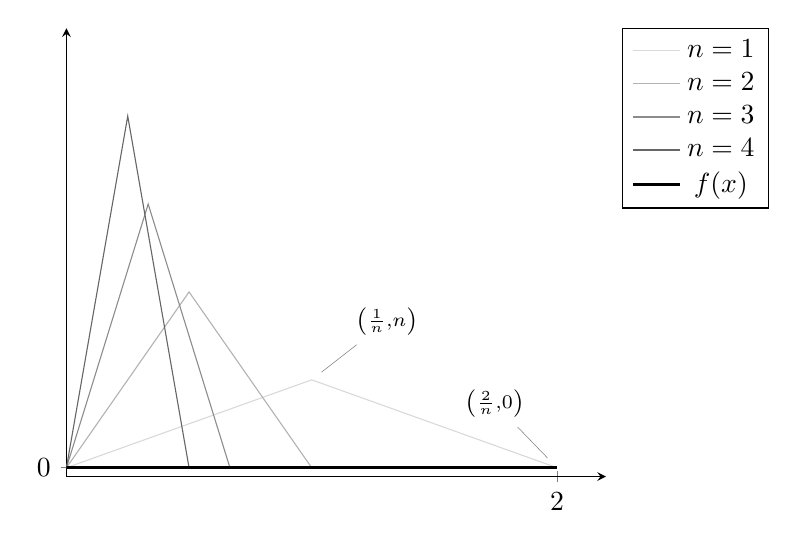
\begin{tikzpicture}
		\begin{axis}[
						enlargelimits,
						legend pos=outer north east,
						axis x line=bottom,axis y line=middle,
						xmin=0,xmax=2.2,ymin=-0.1,ymax=5,ytick={0},xtick={2}
					]
			\addplot [color=black!15!white] coordinates {(0,0) (1/1,1) (2/1,0)};
			\addplot [color=black!30!white] coordinates {(0,0) (1/2,2) (2/2,0)};
			\addplot [color=black!45!white] coordinates {(0,0) (1/3,3) (2/3,0)};
			\addplot [color=black!60!white] coordinates {(0,0) (1/4,4) (2/4,0)};
			\addplot [very thick,color=black,domain=0:2]  {0};
			\node [pin=45:{$\scriptstyle\left(\frac1{n},n\right)$}] at (axis cs:1,1) {};
			\node [pin=120:{$\scriptstyle\left(\frac2{n},0\right)$}] at (axis cs:2,0) {};
			\legend{$n=1$,$n=2$,$n=3$,$n=4$,$f(x)$}
		\end{axis}
	\end{tikzpicture}
	\caption{La successione dell'esempio 3, in $[0,2]$, forma un triangolo di area 1 con l'asse delle ascisse, indipendentemente dal valore di $n$. L'altezza del triangolo aumenta infinitamente al crescere di $n$, mentre la base tende a zero.}
	\label{fig:succ_triangolo}
\end{figure}

\item In $I=[0,1]$, sia
\[
f_n(x)=\begin{cases*}1&se $x=\frac{j}{2^n}$, per $0\leq j\leq 2^n$ intero\\ 0&altrove\end{cases*}.
\]
La funzione limite è la funzione\dots?
\item $f_n(x)=\sqrt{x^2+\frac1{n^2}}$ in $I=\R$, converge puntualmente (figura \ref{fig:succ_iperbole}) alla funzione $f(x)=\abs{x}$.
\begin{figure}
	\tikzsetnextfilename{succ-iperbole}
	\centering
	\begin{tikzpicture}
		\begin{axis}[standard,xtick=\empty,ytick=\empty,xmin=-1.25,xmax=1.25,ymin=-0.5,ymax=2]
			\addplot [samples=500,black!20!white,domain=-1.25:1.25] {sqrt(x^2+1)};
			\addplot [samples=500,black!40!white,domain=-1.25:1.25] {sqrt((x^2)+(1/4))};
			\addplot [samples=500,black!60!white,domain=-1.25:1.25] {sqrt((x^2)+(1/16))};
			\addplot [samples=500,black!80!white,domain=-1.25:1.25] {sqrt((x^2)+(1/36))};
			\addplot [samples=500,black,domain=-1.25:1.25] {abs(x)};
			\node [pin=60:{$\scriptstyle\left(\frac1{n},0\right)$}] at (axis cs:0,1) {};
		\end{axis}
	\end{tikzpicture}
	\caption{Convergenza della funzione $f(x)=\sqrt{x^2+\frac1{n^2}}$ alla funzione limite $f(x)=\abs{x}$, per $n=1,2,4,6$.}
	\label{fig:succ_iperbole}
\end{figure}

\end{enumerate}
Si può studiare se le proprietà della famiglia di funzioni vengano ``ereditate'' dalla funzione limite tramite la convergenza puntuale, ad esempio:
\begin{itemize}
\item se $f_n$ è limitata in $J$ per ogni $n\in\N$, allora anche $f$ è limitata in $J$;
\item se per $\tilde{x}\in J$ esiste il limite delle $f_n(x)$ per $x\to\tilde{x}$, allora $\exists\lim_{x\to\tilde{x}}f(x)$;
\item ulteriormente, per $\tilde{x}\in J$, $\lim_{n\to\pinf}\left(\lim_{x\to\tilde{x}}f_n(x)\right)=\lim_{x\to\tilde{x}}f(x)$;
\item se $f_n$ è continua in $J$ per ogni $n\in\N$, anche $f$ è continua in $J$;
\item se $f_n\in\rie\ab$ $\forall n\in\N$, allora lo è anche $f$, quando ovviamente $f_n\to f$ in $[a,b]$ e, nel caso, valga
\[
\lim_{n\to\pinf}\int_a^bf_n(x)\,\dd x=\int_a^bf(x)\,\dd x;
\]
\item se ogni $f_n$ è derivabile in $x_0\in J$, allora lo è anche $f$ e, nel caso, valga
\[
\lim_{n\to\pinf}f_n'(x_0)=\left(\lim_{n\to\pinf}f_n\right)'(x_0).
\]
\end{itemize}
Nessuna di queste proprietà è valida: gli esempi elencati precedenti forniscono dei buoni controesempi. La funzione limite del punto 1 è illimitata nell'intervallo considerato, mentre le $f_n$ sono limitate per ogni $n$; nel punto 2, la funzione limite non è continua quando tutte le $f_n$ lo sono; nel punto 3, la $f$ tende a 0 per $x\to\pinf$, diversamente dalle $f_n$ che tendono a 1, $\forall n$; nel punto 5 la $f$ non è integrabile secondo Riemann, mentre lo sono tutte le $f_n$, e il punto 4 mostra che l'integrale di tutte le $f_n$ è 1 (geometricamente, è l'area del triangolo formato dalla curva), mentre quello della $f$ è nullo; nel punto 6 infine ogni $f_n$ ha derivata nulla in $x=0$, ma la funzione limite non è nemmeno derivabile in tale punto.

Per garantire queste proprietà, la convergenza puntuale della successione chiaramente non basta: bisogna introdurre un nuovo tipo di convergenza, detta \emph{uniforme}.
\begin{definizione} \label{d:conv_uniforme_succ}
La successione $\{f_n\}$ converge uniformemente alla funzione limite $f$ in $J$ se
\begin{equation} \label{eq:conv_uniforme_succ}
\forall\epsilon>0,\ \exists\overline{n}=\overline{n}(\epsilon)\colon\forall x\in J,\ \forall n\geq\overline{n}\ \abs{f_n(x)-f(x)}<\epsilon.
\end{equation}
\end{definizione}
La definizione è simile a quella della convergenza puntuale se non per il fatto che la scelta di $\overline{n}$ è ora svincolata dal punto $x\in J$, ma è globale in tutto l'insieme $J$; di conseguenza la convergenza uniforme deve sempre essere associata all'insieme in cui accade. Ovviamente la convergenza uniforme implica automaticamente quella puntuale.
Inoltre la differenza tra $f_n$ e la $f$ è certamente, in modulo, sempre minore del suo estremo superiore in $J$, ossia vale sempre $\abs{f_n(x)-f(x)}\leq\sup_{x\in J}\abs{f_n(x)-f(x)}$. Allora per valutare la convergenza uniforme in $J$ è sufficiente calcolare questo estremo superiore, che dovrà annullarsi. Se infatti per la convergenza puntuale doveva verificarsi $\sup_{x\in J}\lim_{n\to\pinf}\abs{f_n(x)-f(x)}=0$, per la convergenza uniforme si ha che
\begin{equation}
\lim_{n\to\pinf}\sup_{x\in J}\abs{f_n(x)-f(x)}=0.
\end{equation}
Si può anche indicare questo estremo superiore con la \emph{norma uniforme}:
\[
\norm{f_n-f}_{\infty,J}=\sup_{x\in J}\abs{f_n(x)-f(x)}.
\]
\paragraph{Esempi}
\begin{itemize}
\item La successione già vista precedentemente $f_n(x)=x^n$ in $[0,1]$ converge puntualmente, però la $\norm{f_n-f}_{\infty,[0,1]}$ vale 0 in $x=1$, perché $f_n(1)=f(1)$, mentre altrove
\[
\norm{f_n-f}_{\infty,[0,1)}=\sup_{0\leq x<1} x^n=\lim_{x\to 1}x^n=1,
\]
e chiaramente $\lim_{n\to\pinf}\neq 0$ quindi la convergenza non è uniforme. Per $\delta>0$ abritrariamente piccolo, però, considerando non più $[0,1]$ ma $[0,1-\delta]$, si ha che 
\[
\norm{f_n-f}_{\infty,[0,1-\delta]}=\sup_{0\leq x\leq 1-\delta} x^n=(1-\delta)^n\to 0,
\]
per $n\to\pinf$, perciò la convergenza è uniforme, dato che $1-\delta$ non dipende nemmeno più da $x$.
\item La successione
\[
f_n(x)=\frac{\arctan\frac{x}{n}}{1+x^2}
\]
converge puntualmente alla funzione identicamente nulla in $\R$. Sia la funzione limite che i termini della successione sono funzioni dispari, quindi si può studiare la convergenza uniforme anche solo per $x\geq 0$. Risulta:
\[
\sup_{x\geq 0}\abs{\frac{\arctan\frac{x}{n}}{1+x^2}}\leq\sup_{x\geq 0}\frac{x}{n}\frac1{1+x^2}=\frac1{n}\sup_{x\geq 0}\frac{x}{1+x^2},
\]
poiché l'arcotangente è in modulo sempre minore del suo argomento, inoltre il termine $1/n$ non dipende da $x$ quindi può essere estratto dall'argomento dell'estremo superiore. La funzione $g(x)=\frac{x}{1+x^2}$ è limitata in $\R$, di conseguenza esiste un numero $c\in\R$ per cui $\abs{g(x)}\leq c$, $\forall x\geq 0$. Dunque
\[
\frac1{n}\sup_{x\geq 0}\frac{x}{1+x^2}\leq\frac{c}{n}
\]
che tende a 0 per $n\to\pinf$, quindi la convergenza è uniforme in tutto $\R$.
\item La convergenza della successione
\[
f_n(x)=\frac{\arctan(nx)}{1+x^2}\quad\to\quad\begin{dcases}\frac{\pi}2\frac{\sgn x}{1+x^2}&x\neq 0\\ 0&x=0\end{dcases}
\]
non è uniforme su tutto $\R$, ma lo è in ogni insieme $A\subset\R\setminus[-\epsilon,\epsilon]$, con $\epsilon>0$, ossia escludendo un intorno dell'origine. Infatti
\begin{multline*}
\sup_{x\geq\epsilon>0}\abs{\frac{\arctan(nx)-\frac{\pi}2\sgn x}{1+x^2}}=\sup_{x\geq\epsilon>0}\frac{\frac{\pi}2-\arctan(nx)}{1+x^2}=\\
=\sup_{x\geq\epsilon>0}\frac{\arctan\frac1{nx}}{1+x^2}=\frac1{1+\epsilon^2}\arctan\frac1{n\epsilon}\to 0
\end{multline*}
per $n\to\pinf$; un risultato analogo si ha per simmetria per $x\leq -\epsilon<0$.
\end{itemize}
Poiché le successioni di funzioni sono comprese in uno spazio metrico completo, quello delle funzioni limitate con la distanza data dalla norma uniforme, in esso si può elaborare la condizione di Cauchy anche per le successioni di funzioni, che sarà sufficiente e necessaria per la convergenza uniforme (dato che la convergenza in tale spazio coincide proprio con la convergenza uniforme)\footnote{Vedere il capitolo \ref{sec:spazi-funz} sugli spazi funzionali.}.
\begin{teorema}
Sia $\{f_n\}$ con $f_n\colon J\to\R$ una successione di funzioni: essa converge uniformemente a $f$ in $J$ se e solo se $\forall\epsilon>0$ $\exists\overline{n}\colon\forall m,n\geq\overline{n}$ si ha $\norm{f_m-f_n}_{\infty,J}<\epsilon$.
\end{teorema}

\section{Proprietà della funzione limite}
Quando la convergenza è uniforme, la funzione limite eredita alcune importanti proprietà dai termini della successione, come mostrato nei seguenti teoremi.
\begin{teorema} \label{t:unif_limitata}
Sia $\{f_n\}$ una successione di funzioni convergente uniformemente a $f$ in $J$ tale che per ogni $n$, $f_n$ è limitata in $J$. Allora anche $f$ è limitata in $J$.
\end{teorema}
\begin{proof}
Se ogni $f_n$ è limitata, vale $\forall n$ che $\abs{f_n(x)}\leq M$.
Per la disuguaglianza triangolare vale inoltre
\[
\abs{f(x)}\leq\abs{f(x)-f_n(x)}+\abs{f_n(x)}\leq\norm{f-f_n}_{\infty,J}+\norm{f_n}_{\infty,J}.
\]
Fissato un $\epsilon>0$ arbitrario, esiste $\overline{n}$ tale per cui $\forall n\geq\overline{n}$, $\norm{f_n-f}_{\infty,J}<\epsilon$. Allora
\[
\sup_{x\in J}\abs{f(x)}\leq\epsilon+\norm{f_{\overline n}}_{\infty,J}.
\]
Poiché il secondo membro è limitato, essendo composto da termini definiti (reali), anche il primo membro è finito, quindi $f(x)$ è limitata in $J$.
\end{proof}
\begin{teorema} \label{t:continuita_conv_uniforme}
Sia $\{f_n\}$ una successione di funzioni definite da $J$ in $\R$, e $x_0\in J$. Se $f_n$ è continua in $x_0$ per ogni $n$, e $\{f_n\}$ converge uniformemente a $f$ in $J$, allora $f$ è a sua volta continua in $x_0$.
\end{teorema}
\begin{proof}
	Per $x\in J$ qualunque, vale la relazione
	\begin{equation}
		\abs{f(x)-f(x_0)}\leq\abs{f_n(x)-f(x)}+\abs{f_n(x)-f_n(x_0)}+\abs{f_n(x_0)-f(x_0)}.
	\end{equation}
	Poiché la convergenza è uniforme, fissato un $\epsilon>0$ esiste $\overline{n}$ per cui $\forall n\geq\overline{n}$ si ha $\norm{f_n-f}_{\infty,J}<\epsilon$, cioè $\abs{f_n(t)-f(t)}<\epsilon$ per ogni $t\in J$; quindi vale anche per i punti $x_0$ e $x$ nella prima equazione. Preso dunque un valore di $n\geq\overline{n}$, ad esempio proprio $\overline{n}$, si ha quindi
	\begin{equation}
		\abs{f(x)-f(x_0)}\leq\epsilon+\abs{f_{\overline n}(x)-f_{\overline n}(x_0)}+\epsilon=\abs{f_{\overline n}(x)-f_{\overline n}(x_0)}+2\epsilon.
	\end{equation}
	La singola funzione $f_{\overline n}(x)$ è continua, per le ipotesi, in $x_0$, quindi in un intorno di tale punto esiste $\delta>0$ tale che per ogni $x\in(x_0-\delta,x_0+\delta)$ si ha $\abs{f_{\overline n}(x)-f_{\overline n}(x_0)}<\epsilon$.
	Allora in tale intorno si ha $\abs{f(x)-f(x_0)}<3\epsilon$, quindi la funzione limite è continua.
\end{proof}
\begin{teorema}[del doppio limite] \label{t:doppio_limite}
Sia $\{f_n\}$ una successione di funzione definite da $J$ a $\R$, e $x_0\in J'$. Se per ogni $n$ esiste $\lim_{x\to x_0}f_n(x)=\ell_n\in\R$, e $\{f_n\}$ converge a $f$ uniformemente in $J$, allora esiste anche $\lim_{n\to\pinf}\ell_n$, che è finito, e coincide con $\lim_{x\to x_0}f(x)$, ossia
\begin{equation} \label{eq:doppio_limite}
\lim_{n\to\pinf}\Big(\lim_{x\to x_0}f_n(x)\Big)=\lim_{x\to x_0}\Big(\lim_{n\to\pinf}f_n(x)\Big).
\end{equation}
\end{teorema}
\begin{teorema} \label{t:scambio_integrale_limite}
Sia $\{f_n\}$ una successione di funzioni definite da $[a,b]$ a $\R$, in cui $f_n$ è integrabile secondo Riemann in $[a,b]$ per ogni $n$, e che converge uniformemente alla funzione $f$ nel medesimo intervallo. Allora anche $f\in\rie\ab$, e vale
\begin{equation} \label{eq:scambio_integrale_limite}
\lim_{n\to\pinf}\int_a^bf_n(x)\,\dd x=\int_a^b\lim_{n\to\pinf}f_n(x)\,\dd x.
\end{equation}
\end{teorema}
La dimostrazione di questo teorema è piuttosto complicata%?
, quindi se ne dimostra una versione più semplice nel corollario seguente.
\begin{corollario}
Sia $\{f_n\}$ una successione di funzioni definite da $[a,b]$ a $\R$, in cui $f_n$ è continua in $[a,b]$ per ogni $n$, e che converge uniformemente alla funzione $f$ nel medesimo intervallo. Allora vale la \eqref{eq:scambio_integrale_limite}.
\end{corollario}
\begin{proof}
Poiché $f_n\in\cont{}\ab$ per ogni $n$, dal teorema \ref{t:continuita_conv_uniforme} segue che anche $f$ lo è, dunque $f\in\rie\ab$. Inoltre si ha
\begin{multline*}
\abs{\int_a^bf_n(x)\,\dd x-\int_a^bf(x)\,\dd x}=\abs{\int_a^b\big[f_n(x)-f(x)\big]\,\dd x}\leq\int_a^b\abs{f_n(x)-f(x)}\,\dd x\leq\\
\leq\int_a^b\norm{f_n-f}_{\infty,[a,b]}\,\dd x=\norm{f_n-f}_{\infty,[a,b]}\int_a^b\dd x=(b-a)\norm{f_n-f}_{\infty,[a,b]},
\end{multline*}
che tende a 0 per $n\to\pinf$, e si ha dunque la \eqref{eq:scambio_integrale_limite}.
\end{proof}
Il teorema non è estendibile a insiemi di integrazione illimitati, come mostrato nel seguente esempio: la successione
\[
f_n(x)=\begin{cases}\frac2{n}-\frac2{n^2}x&x<n\\0&x\geq n\end{cases}
\]
converge uniformemente alla funzione $f(x)=0$ (figura \ref{fig:succ_integrazione_illimitata}). L'integrale di ogni $f_n(x)$ in $[0,\pinf)$ vale 1, per ogni $n$, poiché la curva descritta dalla funzione è un triangolo di base $n$ e altezza $2/n$, ma l'integrale della funzione limite è chiaramente nullo.
\begin{figure}
	\tikzsetnextfilename{succ-integrazione-illimitata}
	\centering
	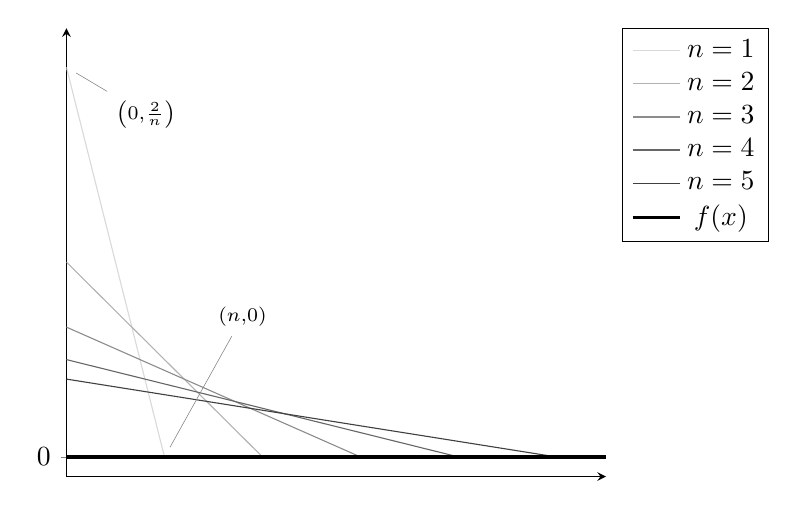
\begin{tikzpicture}
		\begin{axis}[
						enlargelimits,
						legend pos=outer north east,
						axis x line=bottom,axis y line=middle,
						xmin=0,xmax=5.5,ymin=-0.1,ymax=2.2,ytick={0},xtick=\empty
					]
			\addplot [color=black!15!white] coordinates {(0,2/1) (1,0)};
			\addplot [color=black!30!white] coordinates {(0,2/2) (2,0)};
			\addplot [color=black!45!white] coordinates {(0,2/3) (3,0)};
			\addplot [color=black!60!white] coordinates {(0,2/4) (4,0)};
			\addplot [color=black!75!white] coordinates {(0,2/5) (5,0)};
			\addplot [very thick,color=black,domain=0:5.5]  {0};
			\node [pin=-30:{$\scriptstyle\left(0,\frac2{n}\right)$}] at (axis cs:0,2) {};
			\node [pin={[pin distance=1.5 cm]70:{$\scriptstyle(n,0)$}}] at (axis cs:1,0) {};
			\legend{$n=1$,$n=2$,$n=3$,$n=4$,$n=5$,$f(x)$}
		\end{axis}
	\end{tikzpicture}
	\caption{La successione $f_n(x)=\frac2{n}-\frac2{n^2}x$ per $x<n$ e $f_n(x)=0$ per $x\geq n$ forma un triangolo di area 1 con gli assi cartesiani, indipendentemente dal valore di $n$.}
	\label{fig:succ_integrazione_illimitata}
\end{figure}


La derivabilità di una successione di funzioni è una questione più complicata dell'integrabilità: si è già visto in un precedente esempio che anche se la successione converge uniformemente, non è sempre vero che converge anche la successione delle derivate, come per $f_n(x)=\sqrt{x^2+\frac1{n^2}}$, la cui derivata della funzione limite non esiste nemmeno, in $x=0$.
\begin{teorema} \label{t:scambio_derivata_limite}
Sia $\{f_n\}$ una successione di funzioni definite da $[a,b]$ in $\R$ e derivabili in tale intervallo. Se esiste un punto $x_0\in[a,b]$ per cui $\{f_n(x_0)\}$ converge, e se la successione delle derivate $\{f_n'\}$ converge uniformemente in $[a,b]$ ad una funzione $g$, allora esiste una funzione $f\colon[a,b]\to\R$ derivabile, tale che
\begin{itemize}
\item $\{f_n\}$ converga uniformemente a $f$ in $[a,b]$;
\item $f'(x)=g(x)$ in ogni punto $x\in[a,b]$, ossia
\[
\lim_{n\to\pinf}f'_n(x)=\Big(\lim_{n\to\pinf}f_n\Big)'(x).
\]
\end{itemize}
\end{teorema}
Si dà la dimostrazione nel caso particolare in cui $f_n\in\cont{1}\ab$, per ogni $n$.
\begin{proof}
Poiché $f_n'\in\cont{}\ab$, anche $g$ lo è per il teorema \ref{t:continuita_conv_uniforme}. Sapendo che esiste ed è finito il limite
\[
\lim_{n\to\pinf}f_n(x_0)=f(x_0),
\]
si costruisce per ogni punto $x\in[a,b]$ la funzione
\[
f(x)=f(x_0)+\Int_{x_0}^xg(t)\,\dd t.
\]
Essa è derivabile, poiché l'integranda $g$ è continua, $f$ è derivabile per il teorema fondamentale del calcolo integrale \ref{t:tfci1} e la sua derivata è $f'(x)=g(x)$ in $[a,b]$. Inoltre per il medesimo teorema si ha $f_n(x)=f_n(x_0)+\Int_{x_0}^xf_n'(t)\,\dd t$, quindi $\forall x\in[a,b]$ risulta
\[\begin{split}
\abs{f(x)-f_n(x)}	&=\abs{f(x_0)+\Int_{x_0}^xg(t)\,\dd t-f_n(x_0)-\Int_{x_0}^xf_n'(t)\,\dd t}\leq\\
				&\leq\abs{f(x_0)-f_n(x_0)}+\abs{\int_{x_0}^x\big[g(t)-f_n'(t)\big]\,\dd t}\leq\\
				&\leq\abs{f(x_0)-f_n(x_0)}+\abs{x-x_0}\norm{g-f_n'}_{\infty,[a,b]}\leq\\
				&\leq\abs{f(x_0)-f_n(x_0)}+(b-a)\norm{g-f_n'}_{\infty,[a,b]},
\end{split}\]
e poiché per le ipotesi $f_n(x_0)\to f(x_0)$ per $n\to\pinf$, ed $\{f_n'\}$ converge a $g$, si ha che $\{f_n\}$ converge a $f$; la convergenza è infine uniforme in quanto non dipende affatto dalla scelta di $x$, come si nota nell'ultima riga dell'equazione dove la variabile non compare più.
\end{proof}
È importante che la successione $\{f_n\}$ converga almeno in un punto: se si guarda alla successione $f_n(x)=n$, che è costante, la successione delle derivate è $f_n'(x)=0$, cioè sono tutte identicamente nulle ($f_n$ infatti è costante), quindi ovviamente $\{f_n'\}$ converge uniformemente alla funzione identicamente nulla. Ma si nota facilmente che $f_n$ non converge in nessun punto dell'asse reale, nemmeno puntualmente, quindi non esistono nemmeno la funzione limite $f$ né la sua derivata $f'$.

\section{Spazi funzionali}
\label{sec:spazi-funz}
Si indica con la scrittura $\boun{F}{E}$, dove $E\subseteq\R^m$ e $F\subset\R^p$ è chiuso, l'insieme delle funzioni definite in $E$ a valori in $F$ che sono limitate. Su tale insieme si può costruire una struttura spazio metrico, introducendo la distanza
\[
d(\vec f,\vec g)=\sup_{\vec x\in E}\norm{\vec f(\vec x)-\vec g(\vec x)}_F,
\]
dove $\norm{\cdot}_F$ è la norma euclidea in $\R^p$. È un'operazione binaria definita come $d\colon\boun{F}{E}\times\boun{F}{E}\to\R$.
Tale distanza è ben definita, perché tutte le $p$ componenti di $\vec f$ e $\vec g$ sono limitate, quindi $\norm{\vec f(\vec x)}_F\leq M$ e $\norm{\vec g(\vec x)}_F\leq K$ $\forall\vec x\in E$, quindi per la disuguaglianza triangolare risulta $\norm{\vec f(\vec x)-\vec g(\vec x)}_F\leq M+K$, cioè $d(\vec f,\vec g)\leq M+K<\pinf$.
Inoltre soddisfa le proprietà che definiscono una distanza, ossia:
\begin{itemize}
	\item $d(\vec f,\vec g)\ge 0$ $\forall\vec x\in E$ in quanto è una norma euclidea, e $d(\vec f,\vec g)=0$ se e solo se $\norm{\vec f(\vec x)-\vec g(\vec x)}_F=0$ per ogni punto $\vec x\in E$, vale a dire che per tutti i punti $\vec x_0\in E$ risulta $\vec f(\vec x_0)=\vec g(\vec x_0)$, cioè le funzioni coincidono.
	\item $d(\vec f,\vec g)=d(\vec g,\vec f)$ per la simmetria della norma euclidea.
	\item Date tre funzioni $\vec f,\vec g,\vec h\in\boun{F}{E}$, per la disuguaglianza triangolare della norma euclidea si ha
	\begin{equation}
		\begin{split}
			\norm{\vec f(\vec x)-\vec g(\vec x)}_F&\leq\norm{\vec f(\vec x)-\vec h(\vec x)+\vec h(\vec x)-\vec g(\vec x)}_F\leq\\
			&\leq\norm{\vec f(\vec x)-\vec h(\vec x)}_F+\norm{\vec h(\vec x)-\vec g(\vec x)}_F\leq\\
			&\leq d(\vec f,\vec h)+d(\vec h,\vec g).
		\end{split}
	\end{equation}
Poiché quindi per ogni punto $\vec x\in E$ la norma $\norm{\vec f(\vec x)-\vec g(\vec x)}_F$ non supera questa somma delle distanze, anche il suo estremo superiore non la potrà superare, dunque
\[
\sup_{\vec x\in E}\norm{\vec f(\vec x)-\vec g(\vec x)}_F=d(\vec f,\vec g)\leq d(\vec f,\vec h)+d(\vec h,\vec g).
\]
\end{itemize}
Lo spazio $\boun{F}{E}$ può assumere anche la struttura di spazio vettoriale, a seconda che lo sia prima l'insieme $F$ di arrivo. Infatti per la disuguaglianza triangolare la somma di due funzioni limitate è limitata, e analogamente per il prodotto con uno scalare di una funzione limitata. Le immagini dei risultati di queste due operazioni però non appartengono necessariamente ad $F$: questo accade soltanto se l'insieme $F$ è a sua volta uno spazio vettoriale.

Data una successione di funzioni $\vec f_n$ convergente alla funzione limite $\vec f$, secondo tale metrica la convergenza accade se $d(\vec f_n,\vec f)\to 0$ per $n\to\pinf$, cioè se $\vec f_n$ converge uniformemente a $\vec f$.
\begin{teorema}
$\boun{F}{E}$ è uno spazio metrico completo.
\end{teorema}
\begin{proof}
Una successione $\{\vec f_n\}_{n\in\N}$ soddisfa la condizione di Cauchy rispetto alla distanza $d$ se $\forall\epsilon>0$, $\exists N=N(\epsilon)\colon\forall m,n\geq N$ si ha $d(\vec f_n,\vec f_m)<\epsilon$, cioè
\[
\sup_{\vec x\in E}\norm{\vec f_n(\vec x)-\vec f_m(\vec x)}_F<\epsilon,
\]
cioè se e solo se soddisfa il criterio di Cauchy per la convergenza uniforme, quindi $\exists\vec f\colon E\to F$ tale che $\vec f_n\to \vec f$ uniformemente in $E$. Allora $\vec f$ è anche limitata, cioè appartiene a $\boun{F}{E}$.
\end{proof}
Più in generale la funzione limite $\vec f$ avrebbe valori nella chiusura di $F$, ma essa coincide con $F$ stesso poiché è chiuso. Le proprietà dello spazio $\boun{F}{E}$ dipendono fortemente quindi dalla completezza di $F$.

\subsection*{Spazio delle funzioni continue}
Siano $E\subset\R^n$ un insieme compatto e $F\subset\R^p$ chiuso. La scrittura $\mathcal{C}_F(E)$, o anche $\cont{0}_F(E)$, individua lo spazio delle funzioni continue definite da $E$ a $F$.
Per il teorema \ref{t:weierstrass} di Weiestra\ss, tutte le $\vec f\in\cont{0}_F(E)$ sono limitate perché $E$ è compatto, quindi $\cont{0}_F(E)\subset\mathcal B_F(E)$.

Con la distanza $d$ definita per le funzioni limitate, anche $(\cont{0}_F(E),d)$ è uno spazio metrico, ed è anch'esso completo, perché per il teorema \ref{t:continuita_conv_uniforme}, se per ogni $n\in\N$ le funzioni $\vec f_n$ sono continue, allora quando $d(\vec f_n,\vec f)\to 0$ significa che la successione converge uniformemente a $\vec f$, che quindi eredita la continuità; allora se $\{\vec f_n\}_{n\in\N}$ soddisfa la condizione di Cauchy, essa converge in $\cont{0}_F(E)$.

\section{Teorema delle contrazioni}
\begin{definizione}
Dato uno spazio metrico $(X,d)$ e una funzione $T\colon(X,d)\to(X,d)$, $T$ si dice \emph{contrazione} se esiste un valore $k\in[0,1)$ tale per cui
\[
d\big(T(x)-T(y)\big)\leq k d(x,y)
\]
per ogni coppia $x,y\in X$, ossia se $T$ ``contrae'' le distanze (anche non uniformemente) tra $x$ e $y$.
\end{definizione}
Una contrazione è sempre, come si nota facilmente, una funzione lipschitziana di costante $k<1$, quindi è uniformemente continua.
\begin{teorema}[di Banach-Caccioppoli] \label{t:contrazioni}
Sia $(X,d)$ uno spazio metrico completo, e $T\colon X\to X$ una contrazione su $X$. Allora esiste, ed è unico, un \emph{punto fisso} $x^*\in X$ tale per cui $T(x^*)=x^*$.
\end{teorema}
\begin{proof}
Sia $x_0\in X$, $x_1$ l'immagine di $x_0$ attraverso la contrazione $T$ e così via seguendo la regola $x_n=T(x_{n-1})$, per ogni $n\in\N_0$. La distanza tra due elementi della successione costruita in questo modo è
\begin{equation*}
d(x_{n+1},x_n)=d\big(T(x_n),T(x_{n-1})\big)\leq kd(x_n,x_{n-1})\leq k^2d(x_{n-1},x_{n-2})\leq\dots\leq k^nd(x_1,x_0).
\end{equation*}
Dati $m$ e $n$, con $m>n$, si ha per la disguaglianza triangolare che
\begin{equation}
\begin{split}
d(x_m,x_n)\leq	&d(x_m,x_{m-1})+d(x_{m-1},x_{m-2})+\dots+d(x_{n+1},x_n)=\\
				&=\sum_{i=n}^{m-1}d(x_{i+1},x_i)\leq\sum_{i=n}^{m-1}k^id(x_1,x_0)=\\
				&=d(x_1,x_0)k^n\sum_{i=n}^{m-1}k^{i-n}=d(x_1,x_0)k^n\sum_{j=0}^{m-n-1}k^j
\end{split}
\end{equation}
e si ha che
\[
\sum_{j=0}^{m-n-1}k^j\leq\ser{j}k^j=\frac1{1-k},
\]
quindi risulta
\begin{equation}
d(x_m,x_n)\leq\frac{k^n}{1-k}d(x_1,x_0).
\end{equation}
Allora, poiché $k<1$, il secondo termine tende a 0 quindi $\forall\epsilon>0$ $\exists\overline{n}\colon\forall m>n\geq\overline{n}$ si ha $d(x_m,x_n)<\epsilon$, ossia la successione soddisfa la condizione di Cauchy. Dato che lo spazio metrico $(X,d)$ è completo, $\{x_n\}$ converge ad un punto $x^*\in X$ per $n\to\pinf$.
La contrazione $T$ è infine (uniformemente) continua, quindi
\[
T(x^*)=T\Big(\lim_{n\to\pinf}x_n\Big)=\lim_{n\to\pinf} T(x_n)=\lim_{n\to\pinf} x_{n+1}=x^*,
\]
quindi $x^*$ è un punto fisso di $T$; per l'unicità del limite (teorema \ref{t:unicita_limite}) è inoltre unico.
\end{proof}
Non rispettando le ipotesi il teorema non è sempre ancora valido, come ad esempio nello spazio $\R\setminus\{0\}$ con la distanza euclidea: la funzione $f(x)=\frac{x}2$ è una contrazione, ma il suo punto fisso, che sarebbe $x=0$, non appartiene allo spazio.
Anche se $T$ non è una contrazione si hanno degli effetti indesiderati: se $k=1$, infatti le distanze rimangono costanti, come per $g(x)=x+1$, che non ha punti fissi, o per $h(x)=x$ che ne ha infiniti.
\begin{osservazione}
Il teorema \ref{t:contrazioni} non vale se la funzione $T$ è tale per cui $d\big(T(x),T(y)\big)<d(x,y)$, ossia con una disuguaglianza stretta. Infatti, sia $X=[1,\pinf)$: la funzione $f(x)=x+\frac1{x}$ soddisfa questa condizione, ma non ha punti fissi.
\end{osservazione}
